\documentclass[12pt,a4paper]{article}
\usepackage[utf8]{inputenc} % inutile avec XeLaTeX/LuaLaTeX
\usepackage[T1]{fontenc}
\usepackage{amsmath,amssymb,mathrsfs,tikz,times,pifont}
\usepackage{enumitem}
\usepackage{multicol}
\usepackage{lmodern}
\newcommand\circitem[1]{%
\tikz[baseline=(char.base)]{
\node[circle,draw=gray, fill=red!55,
minimum size=1.2em,inner sep=0] (char) {#1};}}
\newcommand\boxitem[1]{%
\tikz[baseline=(char.base)]{
\node[fill=cyan,
minimum size=1.2em,inner sep=0] (char) {#1};}}
\setlist[enumerate,1]{label=\protect\circitem{\arabic*}}
\setlist[enumerate,2]{label=\protect\boxitem{\alph*}}
\everymath{\displaystyle}
\usepackage[left=1cm,right=1cm,top=1cm,bottom=1.7cm]{geometry}
\usepackage[colorlinks=true, linkcolor=blue, urlcolor=blue, citecolor=blue]{hyperref}
\usepackage{array,multirow}
\usepackage[most]{tcolorbox}
\usepackage{varwidth}
\usepackage{float}
\tcbuselibrary{skins,hooks}
\usetikzlibrary{patterns, arrows.meta}
\newtcolorbox{exa}[2][]{enhanced,breakable,before skip=2mm,after skip=5mm,
colback=yellow!20!white,colframe=black!20!blue,boxrule=0.5mm,
attach boxed title to top left ={xshift=0.6cm,yshift*=1mm-\tcboxedtitleheight},
fonttitle=\bfseries,
title={#2},#1,
boxed title style={frame code={
\path[fill=tcbcolback!30!black]
([yshift=-1mm,xshift=-1mm]frame.north west)
arc[start angle=0,end angle=180,radius=1mm]
([yshift=-1mm,xshift=1mm]frame.north east)
arc[start angle=180,end angle=0,radius=1mm];
\path[left color=tcbcolback!60!black,right color = tcbcolback!60!black,
middle color = tcbcolback!80!black]
([xshift=-2mm]frame.north west) -- ([xshift=2mm]frame.north east)
[rounded corners=1mm]-- ([xshift=1mm,yshift=-1mm]frame.north east)
-- (frame.south east) -- (frame.south west)
-- ([xshift=-1mm,yshift=-1mm]frame.north west)
[sharp corners]-- cycle;
},interior engine=empty,
},interior style={top color=yellow!5}}

\usepackage{fancyhdr}
\usepackage{eso-pic}
\usepackage{tkz-tab}
\AddToShipoutPicture{
    \AtTextCenter{%
        \makebox[0pt]{\rotatebox{80}{\textcolor[gray]{0.7}{\fontsize{5cm}{5cm}\selectfont PGB}}}
    }
}

\usepackage{verbatim}

\usepackage{color,soul}

\usepackage{amsmath}
\usepackage{amsfonts}
\usepackage{amssymb}
\usepackage{systeme}
\usepackage{tkz-tab}
\usepackage{tikz}
\usetikzlibrary{arrows}
\newcounter{exemple} % Compteur pour les questions

% Définir la commande pour afficher une question numérotée
\newcommand{\exemple}{%
  \refstepcounter{exemple}%
  \textbf{\textcolor{green}{Exemple \theexemple :}} \ignorespaces
}
%---------------------------------------
\definecolor{myorange}{rgb}{1.0, 0.8, 0.0}

% Définir un compteur pour les exercices d'application
\newcounter{exerciceapp}

% Définir la commande pour afficher un exercice d'application numéroté
\newcommand{\exerciceapp}{%
  \refstepcounter{exerciceapp}%
  \textbf{\textcolor{myorange}{Exercice d'application \theexerciceapp :}} \ignorespaces
}
%--------------------------------------
% Définir un compteur pour les exercices d'application
\newcounter{correction}

% Définir la commande pour afficher un correction exercice d'application numéroté
\newcommand{\correction}{%
  \refstepcounter{correction}%
  \textbf{\textcolor{myorange}{Correction \thecorrection :}} \ignorespaces
}
%--------------------------------------
% Commande pour ajouter du texte en arrière-plan
\usepackage{fancyhdr}
\usepackage{eso-pic}
%\usepackage{tkz-tab}
\AddToShipoutPicture{
    \AtTextCenter{%
        \makebox[0pt]{\rotatebox{80}{\textcolor[gray]{0.7}{\fontsize{5cm}{5cm}\selectfont PGB}}}
    }
}
%This command takes a colour as an optional argument; the default colour is black.
\usetikzlibrary{shapes.geometric,fit}
\newcommand{\myul}[2][black]{\setulcolor{#1}\ul{#2}\setulcolor{black}}
\newcommand\tab[1][1cm]{\hspace*{#1}}

\begin{document}
% En-tête personnalisée
\begin{center}
    \Large\textbf{\underline{\textcolor{red}{Calcul Intégral Ts2}}}\\[-0.1cm]
    \normalsize\textbf{Prof : M. BA} \hfill \textbf{Classe : TS2}\\[-0.1cm]
    \textbf{Année scolaire : 2025 -- 2026}
\end{center}

\section*{\underline{\textbf{\textcolor{red}{I. Intégrale d'une fonction continue: }}}}
\subsection*{\underline{\textbf{\textcolor{red}{1. Introduction :}}}}

Soit \( f \) une fonction continue sur un intervalle \( I \),\( F \) et \( G \) 2 primitives de \( f \) sur \( I \), \( a \) et \( b  \) deux éléments de I. On sait qu'il existe un nombre réel $c$ tel que :$\forall x\in I$, 
 \( G(x) = F(x) + c \)

\underline{\( 
\begin{cases}
G(a) = F(a) + c\\
G(b) = F(b) + c
\end{cases}
\)}

\(
\quad G(b) - G(a) = F(b) - F(a)
\)

Le nombre réel \( F(b) - F(a) \) est donc indépendant de la primitive \( f \) choisie

\subsection*{\underline{\textbf{\textcolor{red}{2. Définition :}}}}

Soit \( f \) une fonction continue sur un intervalle \( I \).
En appelle intégrale de \( a \) à \( b \) de \( f \) le nombre réel \( F(b) - F(a) \) où \( F \) est une primitive de \( f \) sur \( I \) on note :

\(
F(b) - F(a) = \int_{a}^{b} f(x) \, dx = \left[ F(x) \right]_{a}^{b}
\)

\begin{itemize}
    \item \( \int_a^b f(x) \, dx \) se lit ``intégrale ou somme  de $a$ à $b$ de $f(x)dx$''.
    \item \( \left[ F(x) \right]_a^b \) se lit ``\( F(x) \) pris entre \( a \) et \( b \)''.
    \item \( a \) et \( b \) sont les bornes de l'intégrale \( \int_a^b f(x) \, dx \)
        \item Dans l'écriture \( \int_a^b f(x) \, dx \) On peut remplaçer \( x \) par toute autre lettre (sauf \( a \) et \( b \)) on écrit \( \int_a^b f(t) \, dt \) ou \( \int_a^b f(s) \, ds \) ; \( x \) est appelé variable muette.
\end{itemize}

\section*{\textbf{\textcolor{red}{Exemple 1}}}

\(
f(x) = x^2, \quad F(x) = \frac{1}{3} x^3
\)

\(
\begin{aligned}
\int_1^2 f(x) \, dx &= \left[ \frac{1}{3} x^3 \right]_1^2 \\
&= \frac{1}{3} \left[ 2^3 - 1^3 \right] \\
&= \frac{1}{3} \left[ 8 - 1 \right] \\
&= \frac{7}{3}
\end{aligned}
\)

\( \boxed{\int_1^2 f(x) \, dx=\frac{7}{3}} \)

\section*{\textbf{\textcolor{red}{Exemple 2}}}

\(
f(x) = \cos x, \quad F(x) = \sin x
\)

\(
\begin{aligned}
\int_0^{\frac{\pi}{4}} \cos x \, dx &= \left[ \sin x \right]_0^{\frac{\pi}{4}} \\
&= \sin \left( \frac{\pi}{4} \right) - \sin(0) \\
&= \frac{\sqrt{2}}{2} - 0 \\
&= \frac{\sqrt{2}}{2}
\end{aligned}
\)

\( \boxed{\int_0^{\frac{\pi}{4}} \cos x \, dx = \frac{\sqrt{2}}{2}} \)

\section*{\textbf{\textcolor{red}{Propriété 1 }}}
Soit \( f \) une fonction continue sur un intervalle \( I \), \( a \) et \( b \) deux élément de \( I \). On a
\[
\int_a^a f(x) \, dx = 0 \quad;\quad \quad \int_a^b f(x) \, dx = - \int_b^a f(x) \, dx
\]

En effet :

\[
\int_a^b f(x) \, dx = \left[ F(x) \right]_a^b = F(b) - F(a) = 0
\]

\[
\int_a^b f(x) \, dx = \left[ P(x) \right]_a^b = F(b) - F(a) = - \left( P(b) - P(a) \right)=-\int_b^a f(x) \, dx
\]

\subsection*{\underline{\textbf{\textcolor{red}{3. Intégrale et Primitive :}}}}

Soit \( f \) une fonction continue sur \( I \) (intervalle), \( a \in I \), \( F \) primitive de \( f \) sur \( I \), telle que \( F'(x) = f(x) \), et \( F(a) = 0 \). \(F(x) = \int_a^x f(t) \, dt \)

En effet:

\[
\int_a^x f(t) \, dt = F(x) - F(a) = F(x) - 0
\]

\subsection*{\underline{\textbf{\textcolor{red}{4. Interprétation graphique de l'intégrale :}}}}

Soit \( f \) une fonction continue et \textcolor{red}{positive} sur un intervalle \( I \), \( (Cf) \) sa courbe représentative, \( a \) et \( b \in I \) avec \( a < b \).

\(
\int_a^b f(x) \, dx \text{ est l'aire (en unité d'aire) du domaine D délimité par la courbe \( (Cf) \),}\\ \text{l'axe des abscisses \( (OI) \) et les droites d'équation \( x = a \), \( x = b \).}
\)

\(
\text{ Ce domaine est aussi l'ensemble des points $M\begin{pmatrix} x \\ y \end{pmatrix}$  tel que}:
\begin{cases}
a \leq x \leq b \\
0 \leq y \leq f(x)
\end{cases}
\)

\[\text{Ainsi,en notant A(D), aire du domaine et u.a unité d'aire, on a: }
A(D)=\int_a^b f(x) \, dx .u.a 
\]


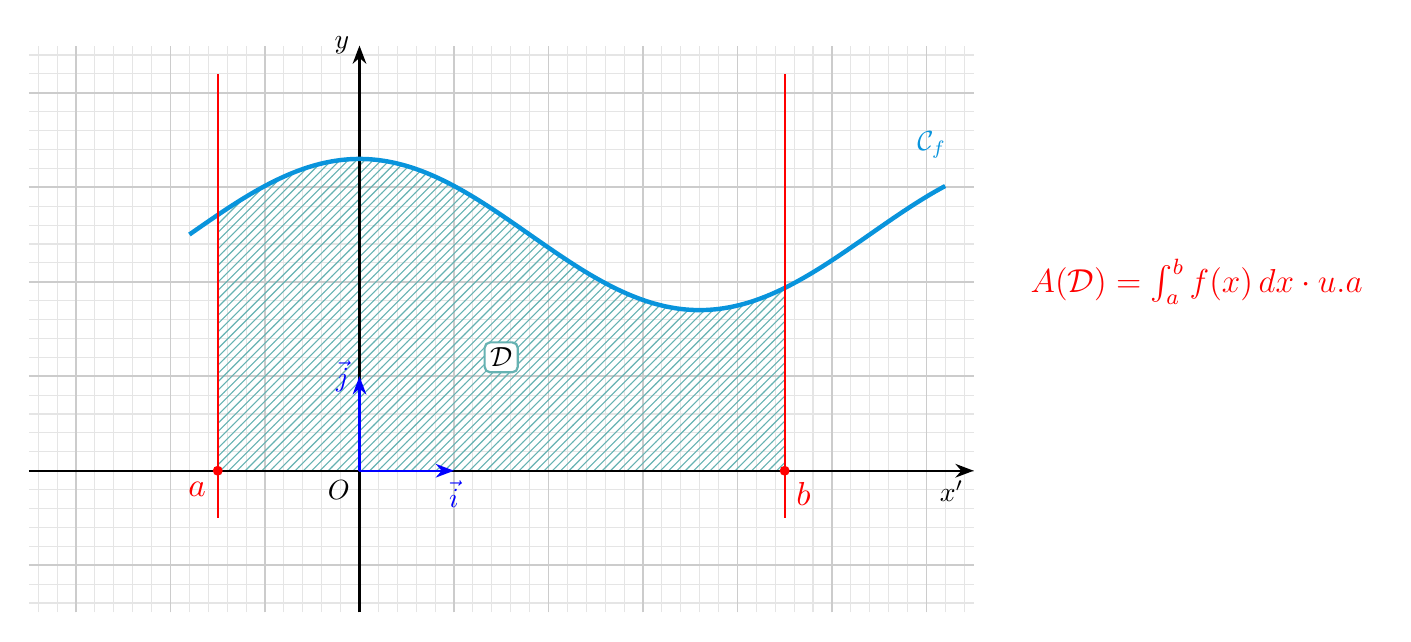
\begin{tikzpicture}[>=Stealth, scale=1.2]

    % --- 1. Grille de fond (style cahier) ---
    \draw[step=0.2cm, gray!20, thin] (-3.5,-1.5) grid (6.5,4.5);
    \draw[step=1cm, gray!40, semithick] (-3.5,-1.5) grid (6.5,4.5);

    % --- 2. Définition de la fonction (courbe sinusoïdale lissée) ---
    \def\fonc{cos(\x*50)*0.8 + 2.5}

    % --- 3. Aire hachurée (sous la courbe entre a et b) ---
    \def\a{-1.5}
    \def\b{4.5}
    
    \path[pattern=north east lines, pattern color=teal!60] 
        (\a,0) -- plot[domain=\a:\b, samples=100] (\x, {\fonc}) -- (\b,0) -- cycle;

    % --- AJOUT : Lettre pour désigner la surface ---
    % On place un node avec un fond blanc légèrement transparent pour couper proprement les hachures
    \node[draw=teal!60, fill=white, rounded corners=2pt, inner sep=2pt, thick] at (1.5,1.2) {$\mathcal{D}$};

    % --- 4. Axes cartésiens ---
    \draw[->, thick] (-3.5,0) -- (6.5,0) node[below left] {$x'$};
    \draw[->, thick] (0,-1.5) -- (0,4.5) node[left] {$y$};
    \node[below left] at (0,0) {$O$};

    % --- 5. Vecteurs directeurs de la base ---
    \draw[->, blue, thick] (0,0) -- (1,0) node[below] {$\vec{i}$};
    \draw[->, blue, thick] (0,0) -- (0,1) node[left] {$\vec{j}$};

    % --- 6. La courbe Cf ---
    \draw[cyan!80!blue, ultra thick, smooth] plot[domain=-1.8:6.2, samples=150] (\x, {\fonc});
    \node[cyan!80!blue, above right] at (5.8, 3.2) {$\mathcal{C}_f$};

    % --- 7. Lignes verticales rouges (bornes a et b) ---
    \draw[red, thick] (\a, -0.5) -- (\a, 4.2);
    \draw[red, thick] (\b, -0.5) -- (\b, 4.2);
    
    % Points et labels sur l'axe x
    \fill[red] (\a,0) circle (1.5pt) node[below left, scale=1.2] {$a$};
    \fill[red] (\b,0) circle (1.5pt) node[below right, scale=1.2] {$b$};
% --- DEPLACEMENT : Formule à droite de la figure ---
    % Placé à x = 9 (à droite de la grille qui se termine à 6.5)
    \node[align=left, text=red, font=\large, anchor=west] at (7.0, 2) {
        $A(\mathcal{D}) = \int_{a}^{b} f(x) \, dx \cdot u.a$
    };
\end{tikzpicture}

\begin{comment}
\begin{center}
   
\includegraphics[scale=0.5]{Screenshot from 2025-04-26 23-30-27.png}
\end{center}
\end{comment}

\section*{\textbf{\textcolor{red}{Remarque}}}
\begin{itemize}
\item[--] Si \( f \) une fonction continue et \textcolor{red}{négative} sur \([a,b]\). La symétrie orthogonale d'axe \( (OI) \) transforme la courbe \(\mathcal{C}_f\) en celle de \( \mathcal{C}'_{-f} \) de f.

Le domaine \( D \) est tranformé en un domaine \( D' \) de meme aire

\( \text{on a :} A(D)=A(D')=\int_a^b -f(x) \, dx .u.a  \)

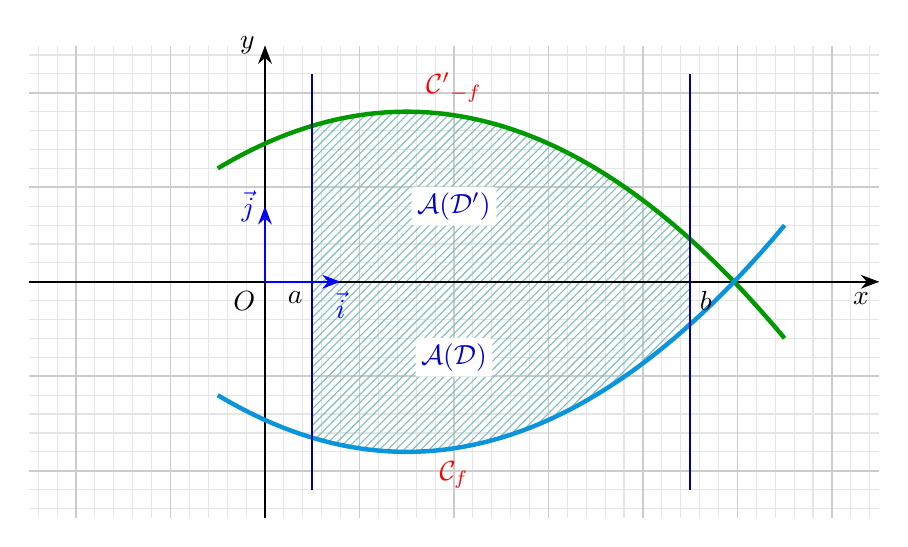
\begin{tikzpicture}[>=Stealth, scale=1.2]

    % --- 1. Grille de fond (style cahier) ---
    \draw[step=0.2cm, gray!20, thin] (-2.5,-2.5) grid (6.5,2.5);
    \draw[step=1cm, gray!40, semithick] (-2.5,-2.5) grid (6.5,2.5);

    % --- 2. Définition des fonctions (valables UNIQUEMENT dans un plot) ---
    \def\foncTop{-0.15*(\x-1.5)*(\x-1.5) + 1.8}
    \def\foncBot{0.15*(\x-1.5)*(\x-1.5) - 1.8}

    % Bornes a et b
    \def\a{0.5}
    \def\b{4.5}

    % --- 3. Aire hachurée complète (correction de la syntaxe ici) ---
    \path[pattern=north east lines, pattern color=teal!50] 
        plot[domain=\a:\b, samples=100] (\x, {\foncTop}) -- 
        plot[domain=\b:\a, samples=100] (\x, {\foncBot}) -- cycle;

    % --- 4. Axes cartésiens ---
    \draw[->, thick] (-2.5,0) -- (6.5,0) node[below left] {$x$};
    \draw[->, thick] (0,-2.5) -- (0,2.5) node[left] {$y$};
    \node[below left] at (0,0) {$O$};

    % --- 5. Vecteurs de la base (i, j) ---
    \draw[->, blue, thick] (0,0) -- (0.8,0) node[below] {$\vec{i}$};
    \draw[->, blue, thick] (0,0) -- (0,0.8) node[left] {$\vec{j}$};

    % --- 6. Les deux courbes ---
    % Courbe du haut (verte)
    \draw[green!60!black, ultra thick, smooth] plot[domain=-0.5:5.5, samples=100] (\x, {\foncTop});
    \node[red, above] at (2,1.8) {$\mathcal{C'}_{-f}$};
    
    % Courbe du bas (bleue/cyan)
    \draw[cyan!80!blue, ultra thick, smooth] plot[domain=-0.5:5.5, samples=100] (\x, {\foncBot});
    \node[red, below] at (2,-1.8) {$\mathcal{C}_f$};

    % --- 7. Droites verticales de délimitation ---
    \draw[blue!60!black, thick] (\a, -2.2) -- (\a, 2.2);
    \draw[blue!60!black, thick] (\b, -2.2) -- (\b, 2.2);
    
    % Noms des bornes
    \node[below left, black] at (\a, 0) {$a$};
    \node[below right, black] at (\b, 0) {$b$};

    % --- 8. Labels de l'aire A(D) ---
    \node[fill=white, inner sep=2pt, rounded corners=1pt, text=blue!80!black] at (2,0.8) {$\mathcal{A}(\mathcal{D'})$};
    \node[fill=white, inner sep=2pt, rounded corners=1pt, text=blue!80!black] at (2,-0.8) {$\mathcal{A}(\mathcal{D})$};

\end{tikzpicture}

\section*{Exemple d'application : Aire sous une courbe négative}

\subsection*{1. Énoncé}
Soit $f$ la fonction définie sur l'intervalle $[0, 3]$ par :
\[ f(x) = x^2 - 3x \]

\begin{enumerate}
    \item Montrer que $f$ est continue et négative sur $[0, 3]$.
    \item Déterminer l'aire $\mathcal{A}(\mathcal{D})$ du domaine $\mathcal{D}$ délimité par la courbe $\mathcal{C}_f$, l'axe des abscisses et les droites d'équations $x = 0$ et $x = 3$.
\end{enumerate}

\subsection*{2. Graphique illustratif}

\begin{center}
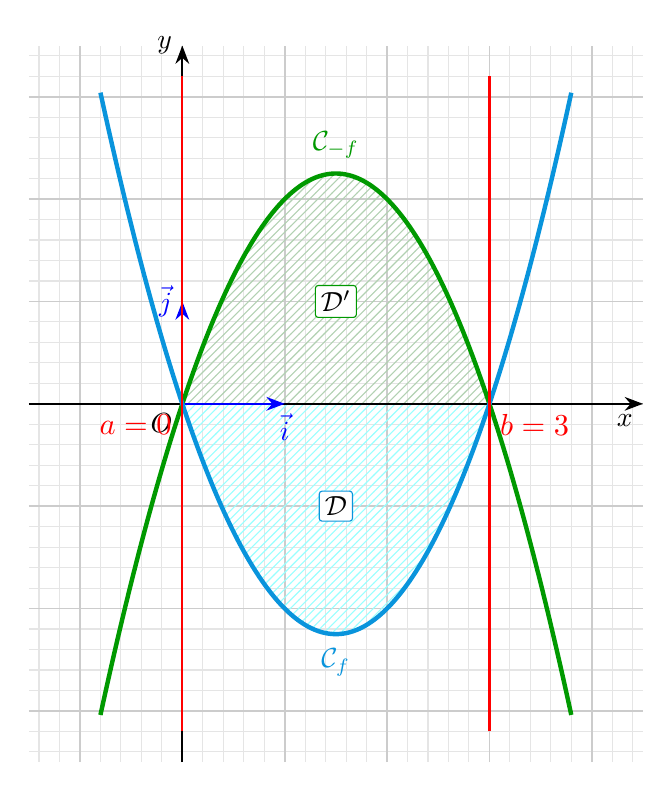
\begin{tikzpicture}[>=Stealth, scale=1.3]

    % --- 1. Grille de fond (style cahier) ---
    \draw[step=0.2cm, gray!20, thin] (-1.5,-3.5) grid (4.5,3.5);
    \draw[step=1cm, gray!40, semithick] (-1.5,-3.5) grid (4.5,3.5);

    % --- 2. Définition des fonctions de l'exemple ---
    \def\foncBot{\x*\x - 3*\x}      % f(x) = x^2 - 3x
    \def\foncTop{-1*(\x*\x - 3*\x)} % -f(x) = -x^2 + 3x

    % Bornes a et b
    \def\a{0.0}
    \def\b{3.0}

    % --- 3. Aires hachurées ---
    % Domaine D' (symétrique, en haut)
    \path[pattern=north east lines, pattern color=green!40!black!30] 
        plot[domain=\a:\b, samples=100] (\x, {\foncTop}) -- (\b,0) -- (\a,0) -- cycle;
        
    % Domaine D (original, en bas)
    \path[pattern=north east lines, pattern color=cyan!40] 
        plot[domain=\a:\b, samples=100] (\x, {\foncBot}) -- (\b,0) -- (\a,0) -- cycle;

    % --- 4. Axes cartésiens ---
    \draw[->, thick] (-1.5,0) -- (4.5,0) node[below left] {$x$};
    \draw[->, thick] (0,-3.5) -- (0,3.5) node[left] {$y$};
    \node[below left] at (0,0) {$O$};

    % --- 5. Vecteurs de la base (i, j) ---
    \draw[->, blue, thick] (0,0) -- (1,0) node[below] {$\vec{i}$};
    \draw[->, blue, thick] (0,0) -- (0,1) node[left] {$\vec{j}$};

    % --- 6. Les deux courbes ---
    % Courbe du haut C_(-f) (verte)
    \draw[green!60!black, ultra thick, smooth] plot[domain=-0.8:3.8, samples=100] (\x, {\foncTop});
    \node[green!60!black, above] at (1.5,2.3) {$\mathcal{C}_{-f}$};
    
    % Courbe du bas C_f (bleue/cyan)
    \draw[cyan!80!blue, ultra thick, smooth] plot[domain=-0.8:3.8, samples=100] (\x, {\foncBot});
    \node[cyan!80!blue, below] at (1.5,-2.3) {$\mathcal{C}_f$};

    % --- 7. Droites verticales de délimitation ---
    \draw[red, thick] (\a, -3.2) -- (\a, 3.2);
    \draw[red, thick] (\b, -3.2) -- (\b, 3.2);
    
    % Noms des bornes
    \node[below left, red, scale=1.1] at (\a, 0) {$a=0$};
    \node[below right, red, scale=1.1] at (\b, 0) {$b=3$};

    % --- 8. Labels des domaines ---
    \node[fill=white, inner sep=2pt, rounded corners=1pt, draw=green!60!black] at (1.5,1.0) {$\mathcal{D}'$};
    \node[fill=white, inner sep=2pt, rounded corners=1pt, draw=cyan!80!blue] at (1.5,-1.0) {$\mathcal{D}$};

\end{tikzpicture}
\end{center}

\subsection*{3. Solution détaillée}

\subsubsection*{Question 1 : Signe et continuité}
\begin{itemize}
    \item \textbf{Continuité :} $f$ est une fonction polynomiale de degré 2. Elle est donc continue sur $\mathbb{R}$, et par restriction, continue sur l'intervalle $[0, 3]$.
    \item \textbf{Signe :} Factorisons l'expression de $f(x)$ : 
    \[ f(x) = x(x - 3) \]
    Pour tout $x \in [0, 3]$, le facteur $x$ est positif ($x \ge 0$) et le facteur $(x - 3)$ est négatif ou nul ($x - 3 \le 0$). Par la règle des signes du produit, on en déduit que pour tout $x \in [0, 3]$ :
    \[ f(x) \le 0 \]
    La fonction $f$ est donc bien \textbf{négative} sur l'intervalle $[0, 3]$.
\end{itemize}

\subsubsection*{Question 2 : Calcul de l'aire par symétrie}
Puisque la fonction $f$ est négative sur $[0,3]$, la symétrie orthogonale d'axe $(OI)$ transforme le domaine $\mathcal{D}$ en un domaine $\mathcal{D}'$ de même aire, situé au-dessus de l'axe des abscisses et délimité par la courbe de la fonction $-f$. 

On a : 
\[ -f(x) = -(x^2 - 3x) = -x^2 + 3x \]

L'aire s'exprime donc par l'intégrale suivante :
\[ \mathcal{A}(\mathcal{D}) = \int_{0}^{3} (-x^2 + 3x) \, dx \cdot u.a \]

Déterminons une primitive $F$ de la fonction $x \mapsto -x^2 + 3x$ :
\[ F(x) = \left[ -\frac{x^3}{3} + \frac{3x^2}{2} \right] \]

En appliquant le théorème fondamental de l'analyse entre les bornes $0$ et $3$ :
\begin{align*}
\mathcal{A}(\mathcal{D}) &= F(3) - F(0) \\
&= \left( -\frac{3^3}{3} + \frac{3 \times 3^2}{2} \right) - \left( -\frac{0^3}{3} + \frac{3 \times 0^2}{2} \right) \\
&= \left( -9 + \frac{27}{2} \right) - 0 \\
&= -\frac{18}{2} + \frac{27}{2} \\
&= \frac{9}{2} \cdot u.a
\end{align*}

\textbf{Conclusion :} L'aire du domaine $\mathcal{D}$ est égale à \textbf{$4,5 \text{ u.a.}$}

\begin{comment}
\begin{center}
   
\includegraphics[scale=0.5]{Screenshot from 2025-04-27 00-00-46.png}
\end{center}
\end{comment}

\item[--] \textbf{si} $f$ continue et \textcolor{red}{negative} ($f \le 0$) sur $[a, c]$ \\
    $f$ continue et positive ($f \ge 0$) sur $[c, b]$

\begin{equation*}
\int_{a}^{b} f(x) \, dx = \int_{a}^{c} f(x) \, dx + \int_{c}^{b} f(x) \, dx
\end{equation*}

\vspace{0.3cm}

\begin{center}
    \setlength{\fboxsep}{10pt} % Espace entre le texte et le cadre
    \definecolor{mathblue}{RGB}{0, 51, 153} % Couleur bleue du cadre manuscrit
    
    \noindent\makebox[\textwidth]{
    \color{mathblue}{\fbox{
        \normalcolor
        $\displaystyle A(\mathcal{D}) = \int_{a}^{c} -f(x) \, dx \cdot u.a + \int_{c}^{b} f(x) \, dx \cdot u.a$
    }}
    }
\end{center}

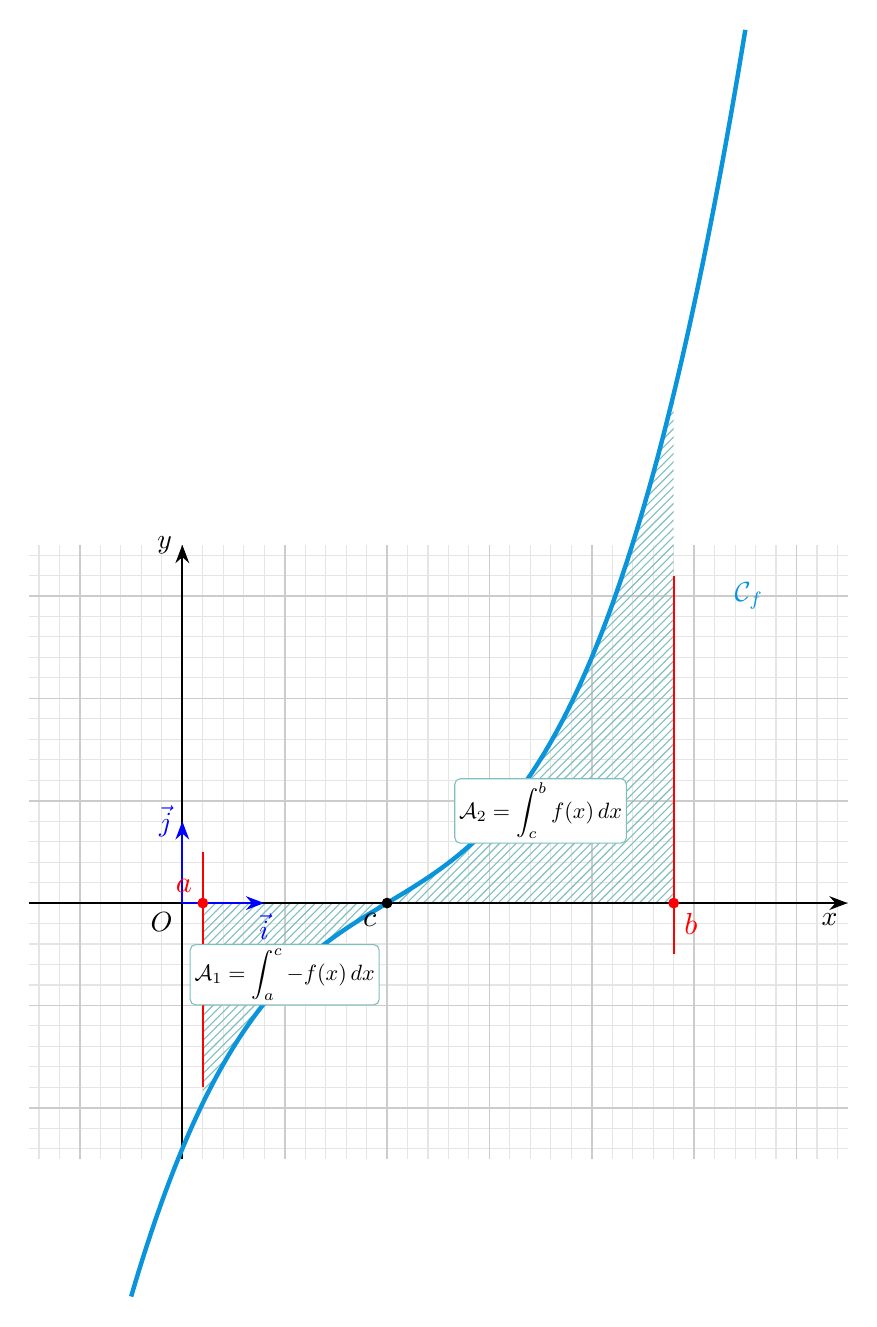
\begin{tikzpicture}[>=Stealth, scale=1.3]

    % --- 1. Grille de fond (style cahier) ---
    \draw[step=0.2cm, gray!20, thin] (-1.5,-2.5) grid (6.5,3.5);
    \draw[step=1cm, gray!40, semithick] (-1.5,-2.5) grid (6.5,3.5);

    % --- 2. Définition de la fonction f ---
    % Une fonction cubique simple qui s'annule exactement en c = 2
    % Négative avant 2, positive après 2
    \def\fonc{0.15*(\x-2)*(\x-2)*(\x-2) + 0.6*(\x-2)}

    % Bornes
    \def\a{0.2}
    \def\c{2.0}
    \def\b{4.8}

    % --- 3. Zones hachurées (Aires) ---
    % Partie 1 : entre a et c (sous l'axe, car f <= 0)
    \path[pattern=north east lines, pattern color=teal!50] 
        plot[domain=\a:\c, samples=100] (\x, {\fonc}) -- (\c,0) -- (\a,0) -- cycle;
        
    % Partie 2 : entre c et b (au-dessus de l'axe, car f >= 0)
    \path[pattern=north east lines, pattern color=teal!50] 
        (\c,0) -- plot[domain=\c:\b, samples=100] (\x, {\fonc}) -- (\b,0) -- cycle;

    % --- 4. Axes cartésiens ---
    \draw[->, thick] (-1.5,0) -- (6.5,0) node[below left] {$x$};
    \draw[->, thick] (0,-2.5) -- (0,3.5) node[left] {$y$};
    \node[below left] at (0,0) {$O$};

    % --- 5. Vecteurs de la base (i, j) ---
    \draw[->, blue, thick] (0,0) -- (0.8,0) node[below] {$\vec{i}$};
    \draw[->, blue, thick] (0,0) -- (0,0.8) node[left] {$\vec{j}$};

    % --- 6. Dessin de la courbe Cf ---
    \draw[cyan!80!blue, ultra thick, smooth] plot[domain=-0.5:5.5, samples=150] (\x, {\fonc});
    \node[cyan!80!blue, right] at (5.3, 3.0) {$\mathcal{C}_f$};

    % --- 7. Lignes verticales de délimitation ---
    \draw[red, thick] (\a, -1.8) -- (\a, 0.5);
    \draw[red, thick] (\b, -0.5) -- (\b, 3.2);
    
    % Marquage des points a, c et b sur l'axe x
    \fill[red] (\a,0) circle (1.5pt) node[above left, scale=1.1] {$a$};
    \fill[black] (\c,0) circle (1.5pt) node[below left, scale=1.1] {$c$};
    \fill[red] (\b,0) circle (1.5pt) node[below right, scale=1.1] {$b$};

    % --- 8. Étiquettes des formules d'aires sous/sur la courbe ---
    % Zone négative (Aire = intégrale de -f)
    \node[fill=white, inner sep=2pt, rounded corners=2pt, draw=teal!50, text=black, scale=0.8] at (1.0, -0.7) 
        {$\displaystyle \mathcal{A}_1 = \int_{a}^{c} -f(x)\,dx$};

    % Zone positive (Aire = intégrale de f)
    \node[fill=white, inner sep=2pt, rounded corners=2pt, draw=teal!50, text=black, scale=0.8] at (3.5, 0.9) 
        {$\displaystyle \mathcal{A}_2 = \int_{c}^{b} f(x)\,dx$};

\end{tikzpicture}


\end{itemize}

\section*{Exercice d'application : Fonction changeant de signe}

\subsection*{1. Énoncé}
Soit $f$ la fonction définie sur l'intervalle $[0, 2]$ par :
\[ f(x) = x^2 - 1 \]

\begin{enumerate}
    \item Étudier le signe de la fonction $f$ sur l'intervalle $[0, 2]$. En déduire la valeur du point de bascule $c$.
    \item Calculer l'intégrale de cette fonction sur $[0, 2]$, c'est-à-dire : $\displaystyle I = \int_{0}^{2} f(x) \, dx$.
    \item Déterminer l'aire géométrique $\mathcal{A}(\mathcal{D})$ du domaine délimité par la courbe $\mathcal{C}_f$, l'axe des abscisses et les droites d'équations $x = 0$ et $x = 2$. Conclure sur la différence avec le résultat précédent.
\end{enumerate}

\subsection*{2. Graphique de l'exercice}

\begin{center}
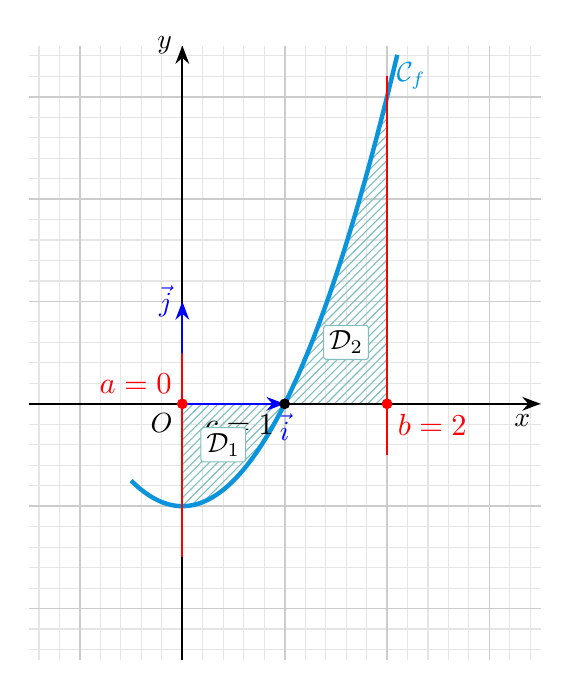
\begin{tikzpicture}[>=Stealth, scale=1.3]

    % --- 1. Grille de fond (style cahier) ---
    \draw[step=0.2cm, gray!20, thin] (-1.5,-2.5) grid (3.5,3.5);
    \draw[step=1cm, gray!40, semithick] (-1.5,-2.5) grid (3.5,3.5);

    % --- 2. Définition de la fonction de l'exercice ---
    \def\fonc{\x*\x - 1} 

    % Bornes
    \def\a{0.0}
    \def\c{1.0}
    \def\b{2.0}

    % --- 3. Zones hachurées (Aires) ---
    % Zone négative (D1) entre 0 et 1
    \path[pattern=north east lines, pattern color=teal!50] 
        plot[domain=\a:\c, samples=100] (\x, {\fonc}) -- (\c,0) -- (\a,0) -- cycle;
        
    % Zone positive (D2) entre 1 et 2
    \path[pattern=north east lines, pattern color=teal!50] 
        (\c,0) -- plot[domain=\c:\b, samples=100] (\x, {\fonc}) -- (\b,0) -- cycle;

    % --- 4. Axes cartésiens ---
    \draw[->, thick] (-1.5,0) -- (3.5,0) node[below left] {$x$};
    \draw[->, thick] (0,-2.5) -- (0,3.5) node[left] {$y$};
    \node[below left] at (0,0) {$O$};

    % --- 5. Vecteurs de la base (i, j) ---
    \draw[->, blue, thick] (0,0) -- (1,0) node[below] {$\vec{i}$};
    \draw[->, blue, thick] (0,0) -- (0,1) node[left] {$\vec{j}$};

    % --- 6. Dessin de la courbe Cf ---
    \draw[cyan!80!blue, ultra thick, smooth] plot[domain=-0.5:2.1, samples=100] (\x, {\fonc});
    \node[cyan!80!blue, right] at (2.0, 3.2) {$\mathcal{C}_f$};

    % --- 7. Lignes verticales de délimitation ---
    \draw[red, thick] (\a, -1.5) -- (\a, 0.5);
    \draw[red, thick] (\b, -0.5) -- (\b, 3.2);
    
    % Marquage des points a, c et b sur l'axe x
    \fill[red] (\a,0) circle (1.5pt) node[above left, scale=1.1] {$a=0$};
    \fill[black] (\c,0) circle (1.5pt) node[below left, scale=1.1] {$c=1$};
    \fill[red] (\b,0) circle (1.5pt) node[below right, scale=1.1] {$b=2$};

    % --- 8. Noms des deux sous-domaines ---
    \node[fill=white, inner sep=2pt, rounded corners=1pt, draw=teal!50] at (0.4, -0.4) {$\mathcal{D}_1$};
    \node[fill=white, inner sep=2pt, rounded corners=1pt, draw=teal!50] at (1.6, 0.6) {$\mathcal{D}_2$};

\end{tikzpicture}
\end{center}

\subsection*{3. Solution rédigée}

\subsubsection*{Question 1 : Étude de signe}
La fonction $f$ est continue sur $[0, 2]$ car c'est une fonction polynôme. 
Résolvons l'équation $f(x) = 0$ :
\[ x^2 - 1 = 0 \iff (x-1)(x+1) = 0 \]
Sur l'intervalle $[0, 2]$, la seule solution est $x = 1$. Le point de bascule est donc \textbf{$c = 1$}.
\begin{itemize}
    \item Pour $x \in [0, 1]$, $x^2 \le 1$ donc $f(x) \le 0$ (\textbf{négative}).
    \item Pour $x \in [1, 2]$, $x^2 \ge 1$ donc $f(x) \ge 0$ (\textbf{positive}).
\end{itemize}

\subsubsection*{Question 2 : Calcul de l'intégrale $I$}
Trouvons une primitive de $f$ définie par $F(x) = \frac{x^3}{3} - x$.
\[ I = \int_{0}^{2} (x^2 - 1) \, dx = \left[ \frac{x^3}{3} - x \right]_{0}^{2} = \left( \frac{8}{3} - 2 \right) - 0 = \frac{2}{3} \]

\subsubsection*{Question 3 : Calcul de l'aire géométrique $\mathcal{A}(\mathcal{D})$}
D'après la propriété du cours (Relation de Chasles adaptée aux signes), l'aire totale est la somme de l'aire des deux sous-domaines $\mathcal{D}_1$ et $\mathcal{D}_2$ :
\[ \mathcal{A}(\mathcal{D}) = \int_{0}^{1} -f(x) \, dx \cdot u.a + \int_{1}^{2} f(x) \, dx \cdot u.a \]
\[ \mathcal{A}(\mathcal{D}) = \int_{0}^{1} (-x^2 + 1) \, dx + \int_{1}^{2} (x^2 - 1) \, dx \]

Calculons séparément chaque partie :
\begin{itemize}
    \item \textbf{Partie négative ($\mathcal{D}_1$) :} $\displaystyle \left[ -\frac{x^3}{3} + x \right]_{0}^{1} = \left(-\frac{1}{3} + 1\right) - 0 = \frac{2}{3}$
    \item \textbf{Partie positive ($\mathcal{D}_2$) :} $\displaystyle \left[ \frac{x^3}{3} - x \right]{1}^{2} = \left(\frac{8}{3} - 2\right) - \left(\frac{1}{3} - 1\right) = \frac{2}{3} - \left(-\frac{2}{3}\right) = \frac{4}{3}$
\end{itemize}

On additionne les deux résultats :
\[ \mathcal{A}(\mathcal{D}) = \frac{2}{3} + \frac{4}{3} = \frac{6}{3} = 2 \cdot u.a \]

\textbf{Conclusion :} L'aire géométrique réelle vaut **$2 \text{ u.a.}$**, tandis que l'intégrale simple calculée à la question 2 ne valait que $\frac{2}{3}$. Cela s'explique par le fait que la partie négative s'est soustraite algébriquement de la partie positive lors du calcul de l'intégrale globale.
 

\section*{\textbf{\textcolor{red}{5. Propriété algébrique de l'intégrale}}}
\subsection*{\textbf{\textcolor{red}{a. Relation de Chasles}}}

Si  \( f \) continue sur un intervalle  \( I \), $a$, $b$ et $c$ trois élément de $K$.

On a:

\[
\int_a^c f(x) \, dx = \int_a^b f(x) \, dx + \int_b^c f(x) \, dx
\]

%\[
%A(D) = \int_a^b -f(x) \, dx.u.A + \int_b^c f(x) \, dx.u.A
%\]

\textbf{Preuve}

\textbf{Interprétation graphique de la relation de Chasles}Voire Ciam pas 298 section 1.2  

\subsubsection*{\underline{\textbf{\textcolor{red}{Exemples}}}}

\(
\begin{aligned}
\int_{-\frac{\pi}{2}}^{\frac{\pi}{2}} \left| \sin(t) \right| \, dt &= \int_{-\frac{\pi}{2}}^{0} -\sin(t) \, dt + \int_{0}^{\frac{\pi}{2}} \sin(t) \, dt\\
&= -\left[\cos(t) \right]_{-\frac{\pi}{2}}^{0} + \left[ \cos(t) \right]_{0}^{\frac{\pi}{2}}\\
&=1+1\\
&=2
\end{aligned}
\)

\( \int_{-\frac{\pi}{2}}^{\frac{\pi}{2}} \left| \sin(t) \right| \, dt = 2 \)

\subsection*{\textbf{\textcolor{red}{b. Linéarité de l'intégrale}}}

Soit \( f \) et \( g \) deux fonctions continues sur \( I \). 

\( \alpha, \beta \) deux réels,  \( a, b \in I \).

On a:

\[
\boxed{\int_a^b \left( \alpha f + \beta g \right)(x) \, dx = \alpha \int_a^b f(x) \, dx + \beta \int_a^b g(x) \, dx}
\]

\section*{\underline{\textbf{\textcolor{red}{Exemples}}}}
Calculer les intégrales suivantes
\[ \int_0^{\frac{\pi}{4}}\cos^{2}(t)dt\]
\section*{\underline{\textbf{\textcolor{red}{Solution}}}}
\( 
\begin{aligned} 
\int_0^{\frac{\pi}{4}}\cos^{2}(t)dt &=\int_0^{\frac{\pi}{4}}\frac{1+\cos(2t)}{2}dt \\
&=\frac{1}{2}\int_0^{\frac{\pi}{4}}1+\cos(2t)dt \\
&=\frac{1}{2}\int_0^{\frac{\pi}{4}}1+\frac{1}{2}\int_0^{\frac{\pi}{4}}\cos(2t)dt \\
\end{aligned}
\)
\subsection*{\underline{\textbf{\textcolor{red}{6. Signe de l'intégrale:}}}}
i)Soit $f$ une fonction continue sur $I$, $a$ et $b\in I$  $(a<b)$
\begin{itemize}
\item si $f>0$ sur $[a,b]$ alors $\int_a^b f(x)dx \geq 0$
\item si $f<0$ sur $[a,b]$ alors $\int_a^b f(x)dx \leq 0$
\end{itemize}
ii)Soit $f$ et $g$ deux fonctions continues sur $I$, $a$ et $b\in I$  $(a<b)$
\begin{itemize}
\item Si $f \leq g$, $\forall x \in[a,b]$ alors $ \int_a^b f(x)dx \leq \int_a^b g(x)dx$
\end{itemize}
\section*{\underline{\textbf{\textcolor{red}{Exemples}}}}

\subsection*{Exemple pour la propriété i) -- Cas d'une fonction positive}
Soit l'intégrale $I = \int_{1}^{2} (x^2 + 3) \, dx$.
\begin{itemize}
    \item \textbf{Étude du signe :} Pour tout $x \in [1, 2]$, on a $x^2 \geq 0$, donc $x^2 + 3 \geq 3 > 0$. La fonction est strictement positive sur l'intervalle d'intégration.
    \item \textbf{Application de la propriété : Bureau de déduction : } Comme les bornes sont ordonnées ($1 < 2$), on en déduit immédiatement que :
    \[ I \geq 0 \]
\end{itemize}

\subsection*{Exemple pour la propriété i) -- Cas d'une fonction négative}
Soit l'intégrale $L = \int_{0}^{3} (-e^x - 1) \, dx$.
\begin{itemize}
    \item \textbf{Étude du signe :} Pour tout $x \in [0, 3]$, l'exponentielle $e^x$ est strictement positive ($e^x > 0$), donc $-e^x < 0$. En retirant encore $1$, on a :
    \[ \forall x \in [0, 3], \quad -e^x - 1 \leq -2 < 0 \]
    La fonction est donc strictement négative sur l'intervalle $[0, 3]$.
    \item \textbf{Application de la propriété :} Puisque l'intervalle respecte l'ordre des bornes ($0 < 3$), la propriété nous garantit sans aucun calcul que :
    \[ L \leq 0 \]
    \item \textbf{Vérification par le calcul :}
    \[ L = \left[ -e^x - x \right]_{0}^{3} = (-e^3 - 3) - (-e^0 - 0) = -e^3 - 3 + 1 = -e^3 - 2 \]
    Comme $e^3 \approx 20,08$, on trouve $L \approx -22,08$, ce qui est bel et bien négatif !
\end{itemize}

\subsection*{Exemple pour la propriété ii) (Comparaison d'intégrales)}
On souhaite comparer, sans les calculer, les deux intégrales suivantes :
\[ J = \int_{0}^{1} x \, dx \quad \text{et} \quad K = \int_{0}^{1} x^2 \, dx \]

\begin{itemize}
    \item \textbf{Comparaison des fonctions :} Sur l'intervalle $[0, 1]$, on sait que multiplier un nombre par lui-même le rend plus petit ou égal (par exemple $0,5^2 = 0,25 \leq 0,5$). On a donc :
    \[ \forall x \in [0, 1], \quad x^2 \leq x \]
    \item \textbf{Application de la propriété :} Les fonctions $x \mapsto x^2$ et $x \mapsto x$ sont continues sur $[0, 1]$ et les bornes sont ordonnées ($0 < 1$). Par croissance de l'intégrale, on obtient directement :
    \[ \int_{0}^{1} x^2 \, dx \leq \int_{0}^{1} x \, dx \quad \implies \quad K \leq J \]
    \item \textbf{Vérification par le calcul :} 
    \[ K = \left[ \frac{x^3}{3} \right]_{0}^{1} = \frac{1}{3} \quad \text{et} \quad J = \left[ \frac{x^2}{2} \right]_{0}^{1} = \frac{1}{2} \]
    On constate bien que $\frac{1}{3} \leq \frac{1}{2}$, la propriété est vérifiée.
\end{itemize}

\subsection*{\underline{\textbf{\textcolor{red}{Remarque :}}}}

Soit \( f \) une fonction continue sur \( I \), \( a \) et \( b \in I \), tel que \( a \leq b \).

On a: \( -|f| \leq |f| \leq |f| \text{ sur } [a ; b] ; \text{on en déduit que} : \left| \int_a^b f(x) \, dx \right| \leq \int_a^b |f(x)| \, dx\)

\subsection*{\underline{\textbf{\textcolor{red}{7. Inégalité de la moyenne :}}}}

\textbf{i)} Soit \( f \) une fonction continue sur \( I \) (intervalle) \( a \) et \( b \in I \)

Si \( m \) et \( M \) sont deux nombres réels tels que \( x \in [a, b] \) \( m \leq f(x) \leq M \),  

\[
\textbf{alors }m (b - a) \leq \int_a^b f(x) \, dx \leq M(b - a)
\]  
\textbf{ii)} Soit \( f \) une fonction continue sur un intervalle \( I \) tel que \( a \leq b \in I \).

Si  \( M \) deux réels tels que \(|f(x)| \leq M, \quad \forall x \in [a,b]\)

On en déduit :

\[
\left| \int_a^b f(x) \, dx \right| \leq M (b-a)
\]

\subsection*{\underline{\textbf{\textcolor{red}{8. Valeur moyenne d'une fonction :}}}}

Soit \( f \) une fonction continue sur un intervalle \( [a, b] \), on appelle valeur moyenne de \( f \) sur \( [a, b] \) le nombre réel \( u \) défini par :

\[
u = \frac{1}{b - a} \int_a^b f(x) \, dx
\]
\section*{\underline{\textbf{\textcolor{red}{II. Techniques de calcul intégral}}}}

\subsection*{\underline{\textbf{\textcolor{red}{1. Primitives usuelles :}}}}

Le tableau suivant reprend quelques résultats concernant les primitives, vus dans les chapitres précédents. Dans ce tableau, \( u \) désigne une fonction dérivable sur un intervalle \( K \), \( v \) une fonction dérivable sur un intervalle contenant \( u(K) \) et \( \alpha \) un nombre réel différent de \( -1 \).

\begin{tabular}{|c|c|c|c|c|}
\hline
\textbf{Fonction} & \( \frac{u'}{u} \) & \( u' e^u \) & \( u' u^\alpha \) & \( u' \cdot v' \circ u \) \\
\hline
\textbf{Primitive} & \( \ln |u| \) & \( e^u \) & \( \frac{1}{\alpha + 1} u^{\alpha + 1} \) & \( v \circ u \) \\
\hline
\textbf{Commentaires} & \( u \neq 0 \) sur \( K \) & - & \( u > 0 \) sur \( K \) & - \\
\hline
\end{tabular}

\subsection*{Examples}

\begin{itemize}
    \item \( \int_0^1 \left( t^3 + 2t + 1 \right) \, dt = \left[ \frac{t^4}{4} + t^2 + t \right]_0^1 = \frac{9}{4} \)
    
    \item \( \int_0^{\frac{\pi}{4}} \sin \left( 2t + \frac{\pi}{2} \right) \, dt = \left[ -\frac{1}{2} \cos \left( 2t + \frac{\pi}{2} \right) \right]_0^{\frac{\pi}{4}} = \frac{1}{2} \)
    
    \item \( \int_0^{\frac{1}{2}} \frac{2t}{t^2 - 1} \, dt = \left[ \ln |t^2 - 1| \right]_0^{\frac{1}{2}} = \ln \frac{3}{4} \)
    
    \item \( \int_0^{\frac{\pi}{2}} \cos t \, e^{\sin t} \, dt = \left[ e^{\sin t} \right]_0^{\frac{\pi}{2}} = e - 1 \)
\end{itemize}
\subsection*{\underline{\textbf{\textcolor{red}{2. Intégration par parties : }}}}
Soit \( u \) et \( v \) deux fonctions dérivables sur un intervalle \( K \) telles que les dérivées \( u' \) et \( v' \) sont continues sur \( K \), \( a \) et \( b \) deux éléments de \( K \).

On a :

\[
\int_a^b u(t) v'(t) \, dt = \left[ u(t) v(t) \right]_a^b - \int_a^b u'(t) v(t) \, dt
\]

\subsection*{Examples}

\begin{itemize}
    \item Calculer : \( \int_1^2 \ln t \, dt \).
    
    Posons : \( u(t) = \ln t \) et \( v'(t) = 1 \).
    
    On a : \( u'(t) = \frac{1}{t} \) ; choisissons : \( v(t) = t \).
    
    \( u' \) et \( v' \) sont continues sur \( [1 ; 2] \).
    
    Donc :
    \[
    \int_1^2 \ln t \, dt = \left[ t \ln t \right]_1^2 - \int_1^2 dt
    \]
    \[
    = \left[ t \ln t \right]_1^2 - \left[ t \right]_1^2
    \]
    \[
    = \left[ 2 \ln 2 - 2 \right] - \left[ 1 \ln 1 - 1 \right] = 2 \ln 2 - 1
    \]
    
    \item Calculer : \( \int_0^{\frac{\pi}{2}} t \cos t \, dt \).
    
    Posons : \( u(t) = t \) et \( v'(t) = \cos t \).
    
    On a : \( u'(t) = 1 \) ; choisissons : \( v(t) = \sin t \).
    
    \( u' \) et \( v' \) sont continues sur \( [0 ; \frac{\pi}{2}] \).
    
    Donc :
    \[
    \int_0^{\frac{\pi}{2}} t \cos t \, dt = \left[ t \sin t \right]_0^{\frac{\pi}{2}} - \int_0^{\frac{\pi}{2}} \sin t \, dt
    \]
    \[
    = \left[ t \sin t \right]_0^{\frac{\pi}{2}} - \left[ - \cos t \right]_0^{\frac{\pi}{2}}
    \]
    \[
    = \left[ \frac{\pi}{2} \sin \frac{\pi}{2} - 0 \right] - \left[ - \cos \frac{\pi}{2} + \cos 0 \right]
    \]
    \[
    = \left[ \frac{\pi}{2} \times 1 \right] - \left[ - 0 + 1 \right] = \frac{\pi}{2} - 1
    \]
\end{itemize}

\begin{tcolorbox}[
    colframe=red, % Bordure rouge
    colback=white, % Fond blanc
    title=\textbf{Remarque : Choix de $u(x)$ (Méthode ALPES)}, 
    coltitle=white, % Texte du titre en blanc sur fond rouge
    fonttitle=\bfseries,
    arc=2mm % Angles légèrement arrondis
]
Pour effectuer une intégration par parties (IPP) efficace, le choix de la fonction $u(x)$ à dériver se fait judicieusement grâce au moyen mnémotechnique \textbf{ALPES}. 

En lisant le mot de gauche à droite, la première fonction rencontrée dans l'intégrale définit $u(x)$ :
\begin{itemize}
    \item[\textbf{A} :] \textbf{A}rc (Fonctions réciproques : $\arctan$, $\arcsin$...)
    \item[\textbf{L} :] \textbf{L}ogarithme ($\ln$)
    \item[\textbf{P} :] \textbf{P}olynôme ($x$, $x^2-1$...)
    \item[\textbf{E} :] \textbf{E}xponentielle ($e^x$...)
    \item[\textbf{S} :] \textbf{S}inus / Cosinus (Fonctions trigonométriques)
\end{itemize}
\textit{Exemple :} Dans $\int x e^x \,dx$, le polynôme ($x$) passe avant l'exponentielle ($e^x$) dans le mot A-\textbf{P}-\textbf{E}-S, on pose donc $u(x) = x$.
\end{tcolorbox}

\subsection*{\underline{\textbf{\textcolor{red}{3. Intégration de fonctions paires, impaires, périodiques : }}}}
\subsubsection*{\underline{\textcolor{red}{Propriété 1 :}}}
Soit \(f\) une fonction continue sur un intervalle \(I\) symétrique par rapport à \(0\).

\( \forall \alpha \in I \), on a:

\begin{itemize}
    \item Si \(f\) est paire, \( \int_{-\alpha}^{\alpha}f(x)dx = 2 \int_{0}^{\alpha}f(x)dx \)
    \item Si \(f\) est impaire, \( \int_{-\alpha}^{\alpha}f(x)dx =  0 \)
\end{itemize}
\subsection*{Examples}
CIAM
\subsubsection*{\underline{\textcolor{red}{Propriété 2 :}}}
Soit \(f\) une fonction continue sur \( \mathbb{R} \) et périodique, de période \(p\).

Pour tous nombres réel \(a\) et \(b\), on a:

\begin{itemize}
    \item Si \(f\) est paire, \( \int_{a+p}^{b+p}f(x)dx = \int_{a}^{b}f(x)dx \)
    \item Si \(f\) est impaire, \( \int_{a}^{a+p}f(x)dx =  \int_{0}^{p}f(x)dx = 0 \)
\end{itemize}
\subsection*{Examples}
CIAM
\section*{\underline{\textbf{\textcolor{red}{III. Application du calcul intégral}}}}
\subsubsection*{\underline{\textcolor{red}{Propriété :}}}
Soit \(f\) et \(g\) deux fonctions continues sur un intervalle \(I\), \( (\mathcal{C}_f) \) et \( (\mathcal{C}_g) \) leurs réprésentations graphiques respectives \(a\) et \(b\) deux éléments de \(I\) (\(a<b\))
Lorsque \(f \leq g\) sur \( [a;b] \), l'aire du domaine \(D\) délimité par \( (\mathcal{C}_f) \), \( (\mathcal{C}_g) \) et les droites d'équations \( x=a \) et \( x=b \) est: \(\mathcal{A}(D)=\int_{a}^{b} [g(x)-g(x)]dx \)

\textbf{Voir dessin}
\subsection*{Examples}
CIAM
\end{document}
